%%This is a very basic article template.
%%There is just one section and two subsections.
\documentclass{VLKlauck}
\usepackage{graphicx}
\usepackage{array}
\author[]{Christian Holl (24296)}
\institute[HTW Aaalen - Elektronik und Informatik]
{
	Studiengang Computer Controlled Systems\\
	Hochschule Aalen - Technik und Wirtschaft
}

\graphicspath{{./img/}}

\title[]{Online Symbolerkennung durch Datenfusion einer 3D und einer Farbkamera für einen autonomen Roboter}

\newcolumntype{S}{>{\centering\arraybackslash} m{.4\linewidth} }
	

\date[]{\today}  

\usepackage[right]{eurosym}
    
\begin{document}
\maketitle

  \section{Einleitung}
  \subsection{Aufgabenstellung}
	\begin{frame}{Aufgabenstellung}   
		\begin{itemize}
		  \item 3D-Kamera: Microsoft Kinect
		  \item Software: ROS (Robot Operating System \url{http://www.ros.org})
		  \item Finden von Oberflächen mit passenden Eigenschaften:
		 	 \begin{itemize}
		    	\item Ausrichtung (senkrecht zum Betrachter) 
		    	\item Größe 
		    	\item Ort
		    	\item Entfernung   
			\end{itemize}
		  \item Durchsuchen der Oberflächen nach bekannten Symbolen
		\end{itemize}
		Hintergrund: Schnelleres Auffinden von Schildern in Kamerabildern
	\end{frame} 
	\subsection{Funktionsweise Kinect} 
	\begin{frame}{Kinect: Übersicht}
		Tiefenkamera und Farbkamera in einem (Preis \textasciitilde \EUR{110})  
		
		\begin{tabular}{cc}
			Übersicht 								   & Bild IR-Sensor\\
			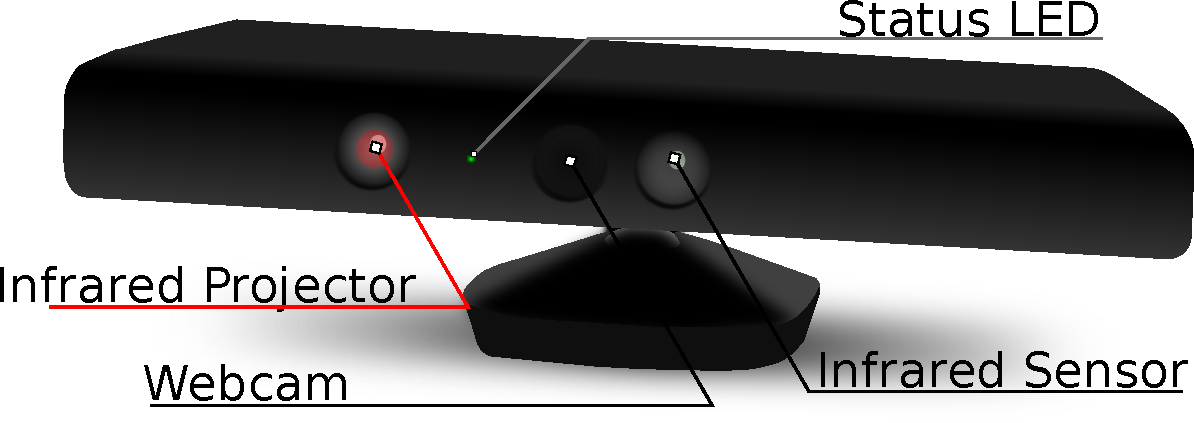
\includegraphics[scale=0.3]{Kinect.pdf}  & 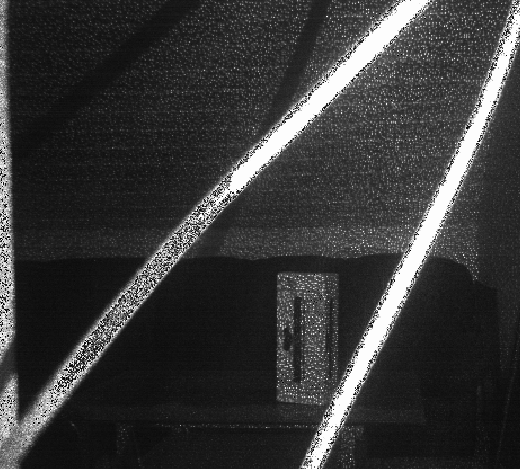
\includegraphics[scale=0.4]{ir_kinect.png}\\	
		\end{tabular}  
		
	\end{frame}
	

	\begin{frame}{Kinect Funktionsweise} 
		
		\begin{tabular}{SS}
			Laserscanner							   & Kinect\\
			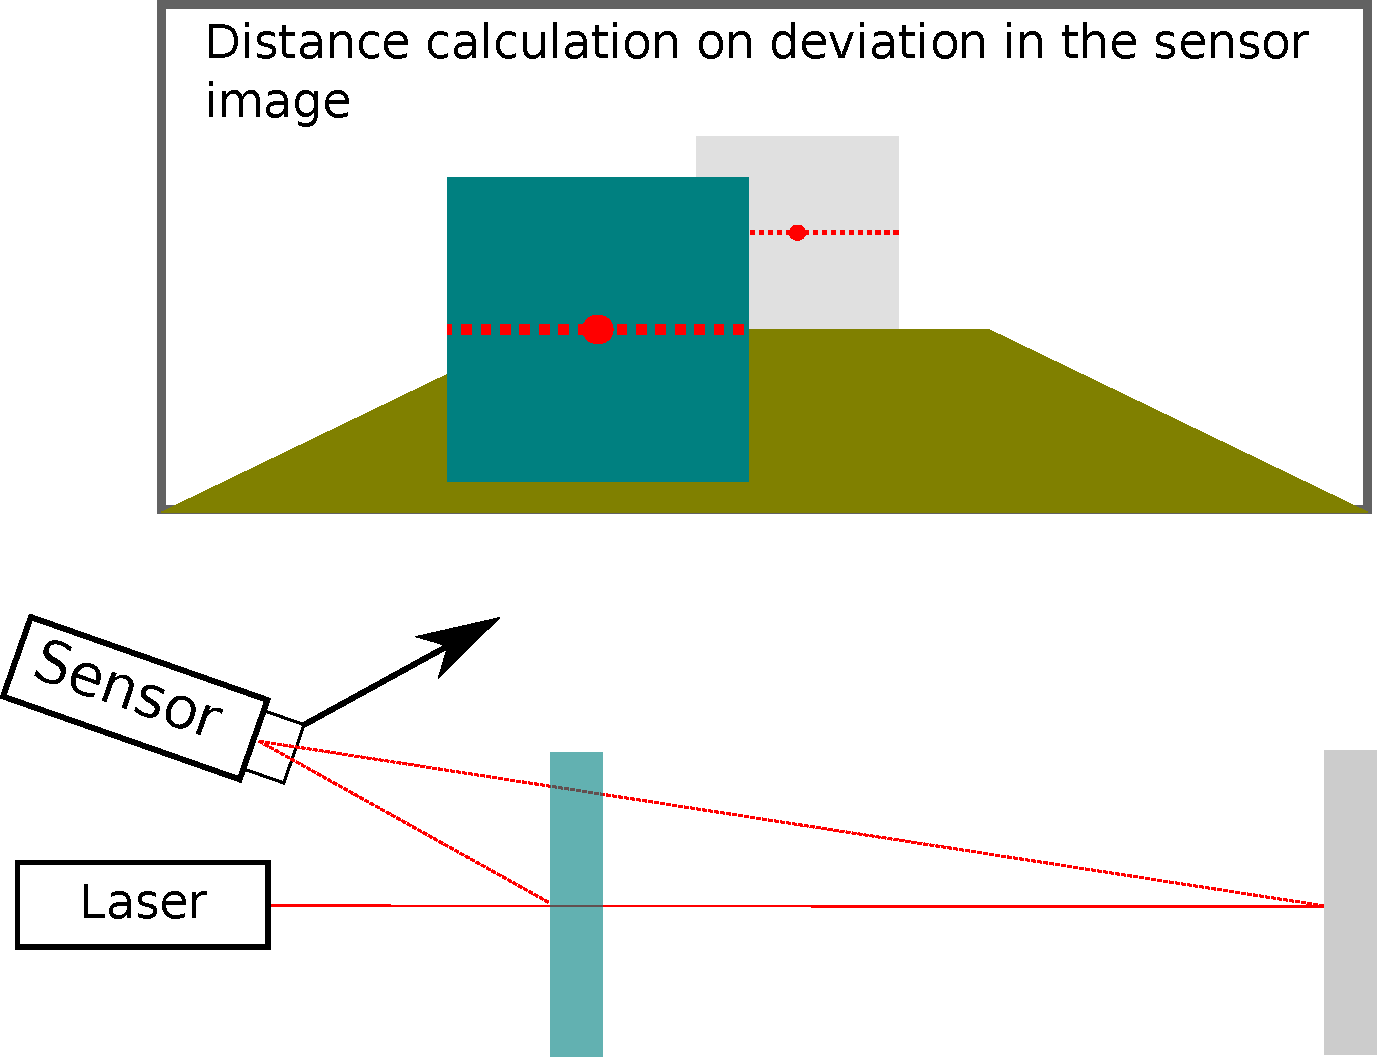
\includegraphics[scale=0.18]{laserScannerPrinciple.pdf}  & 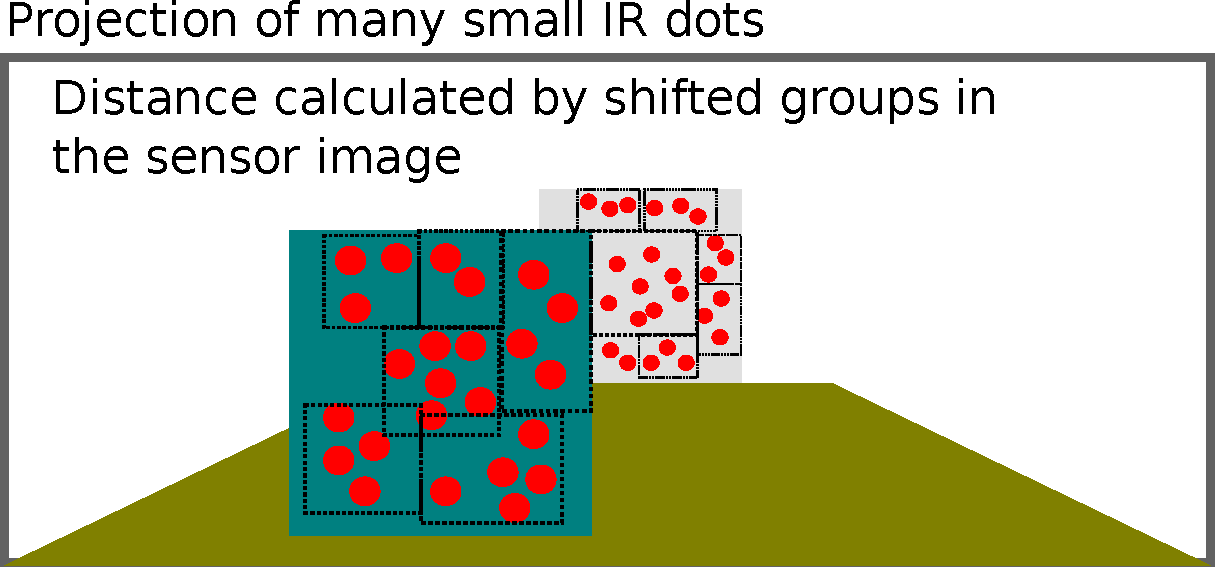
\includegraphics[scale=0.18]{kinect_principle.pdf}\\	
		\end{tabular} 
	\end{frame}
	
	\subsection{ROS(Publisher Subscriber Pattern)}
	\begin{frame}{ROS(Publisher Subscriber Pattern)}
		\centering
			Beispiel Realität\\					   
			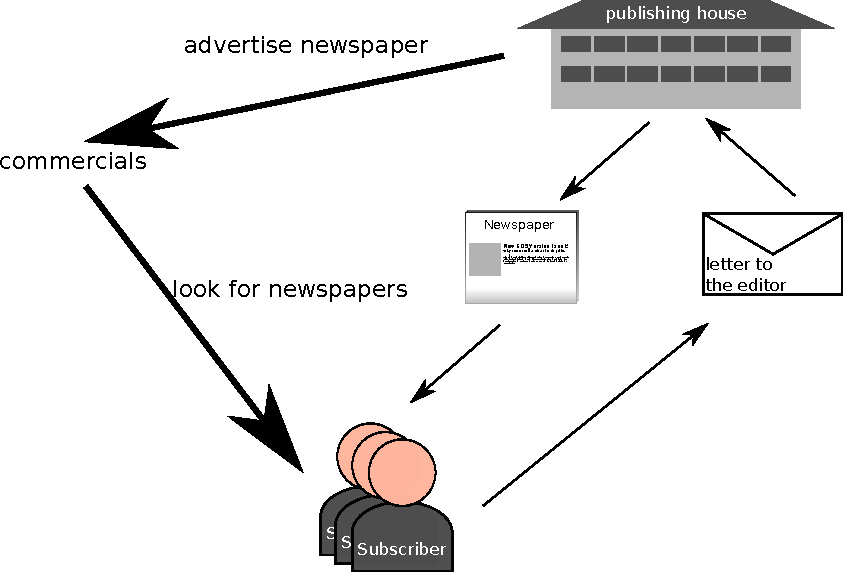
\includegraphics[scale=0.5]{PS_Newspaper.pdf}
	\end{frame}
	
 	\begin{frame}{ROS(Publisher Subscriber Pattern)}
		\centering
		Beispiel ROS\\			   
		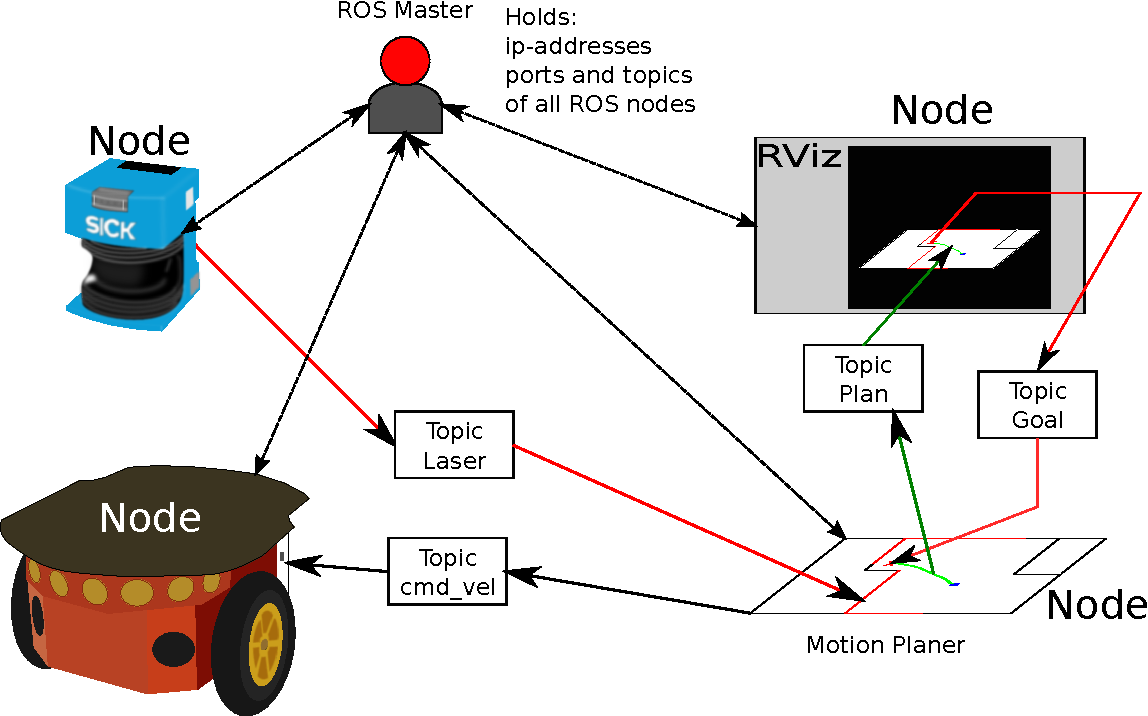
\includegraphics[scale=0.5]{PS_ROS.pdf}
	\end{frame}
	
	\subsection{Mechanik}
	\begin{frame}{Mechanik}
		\begin{tabular}{cc}
			Schilder 								   & Änderungen am Roboter\\
			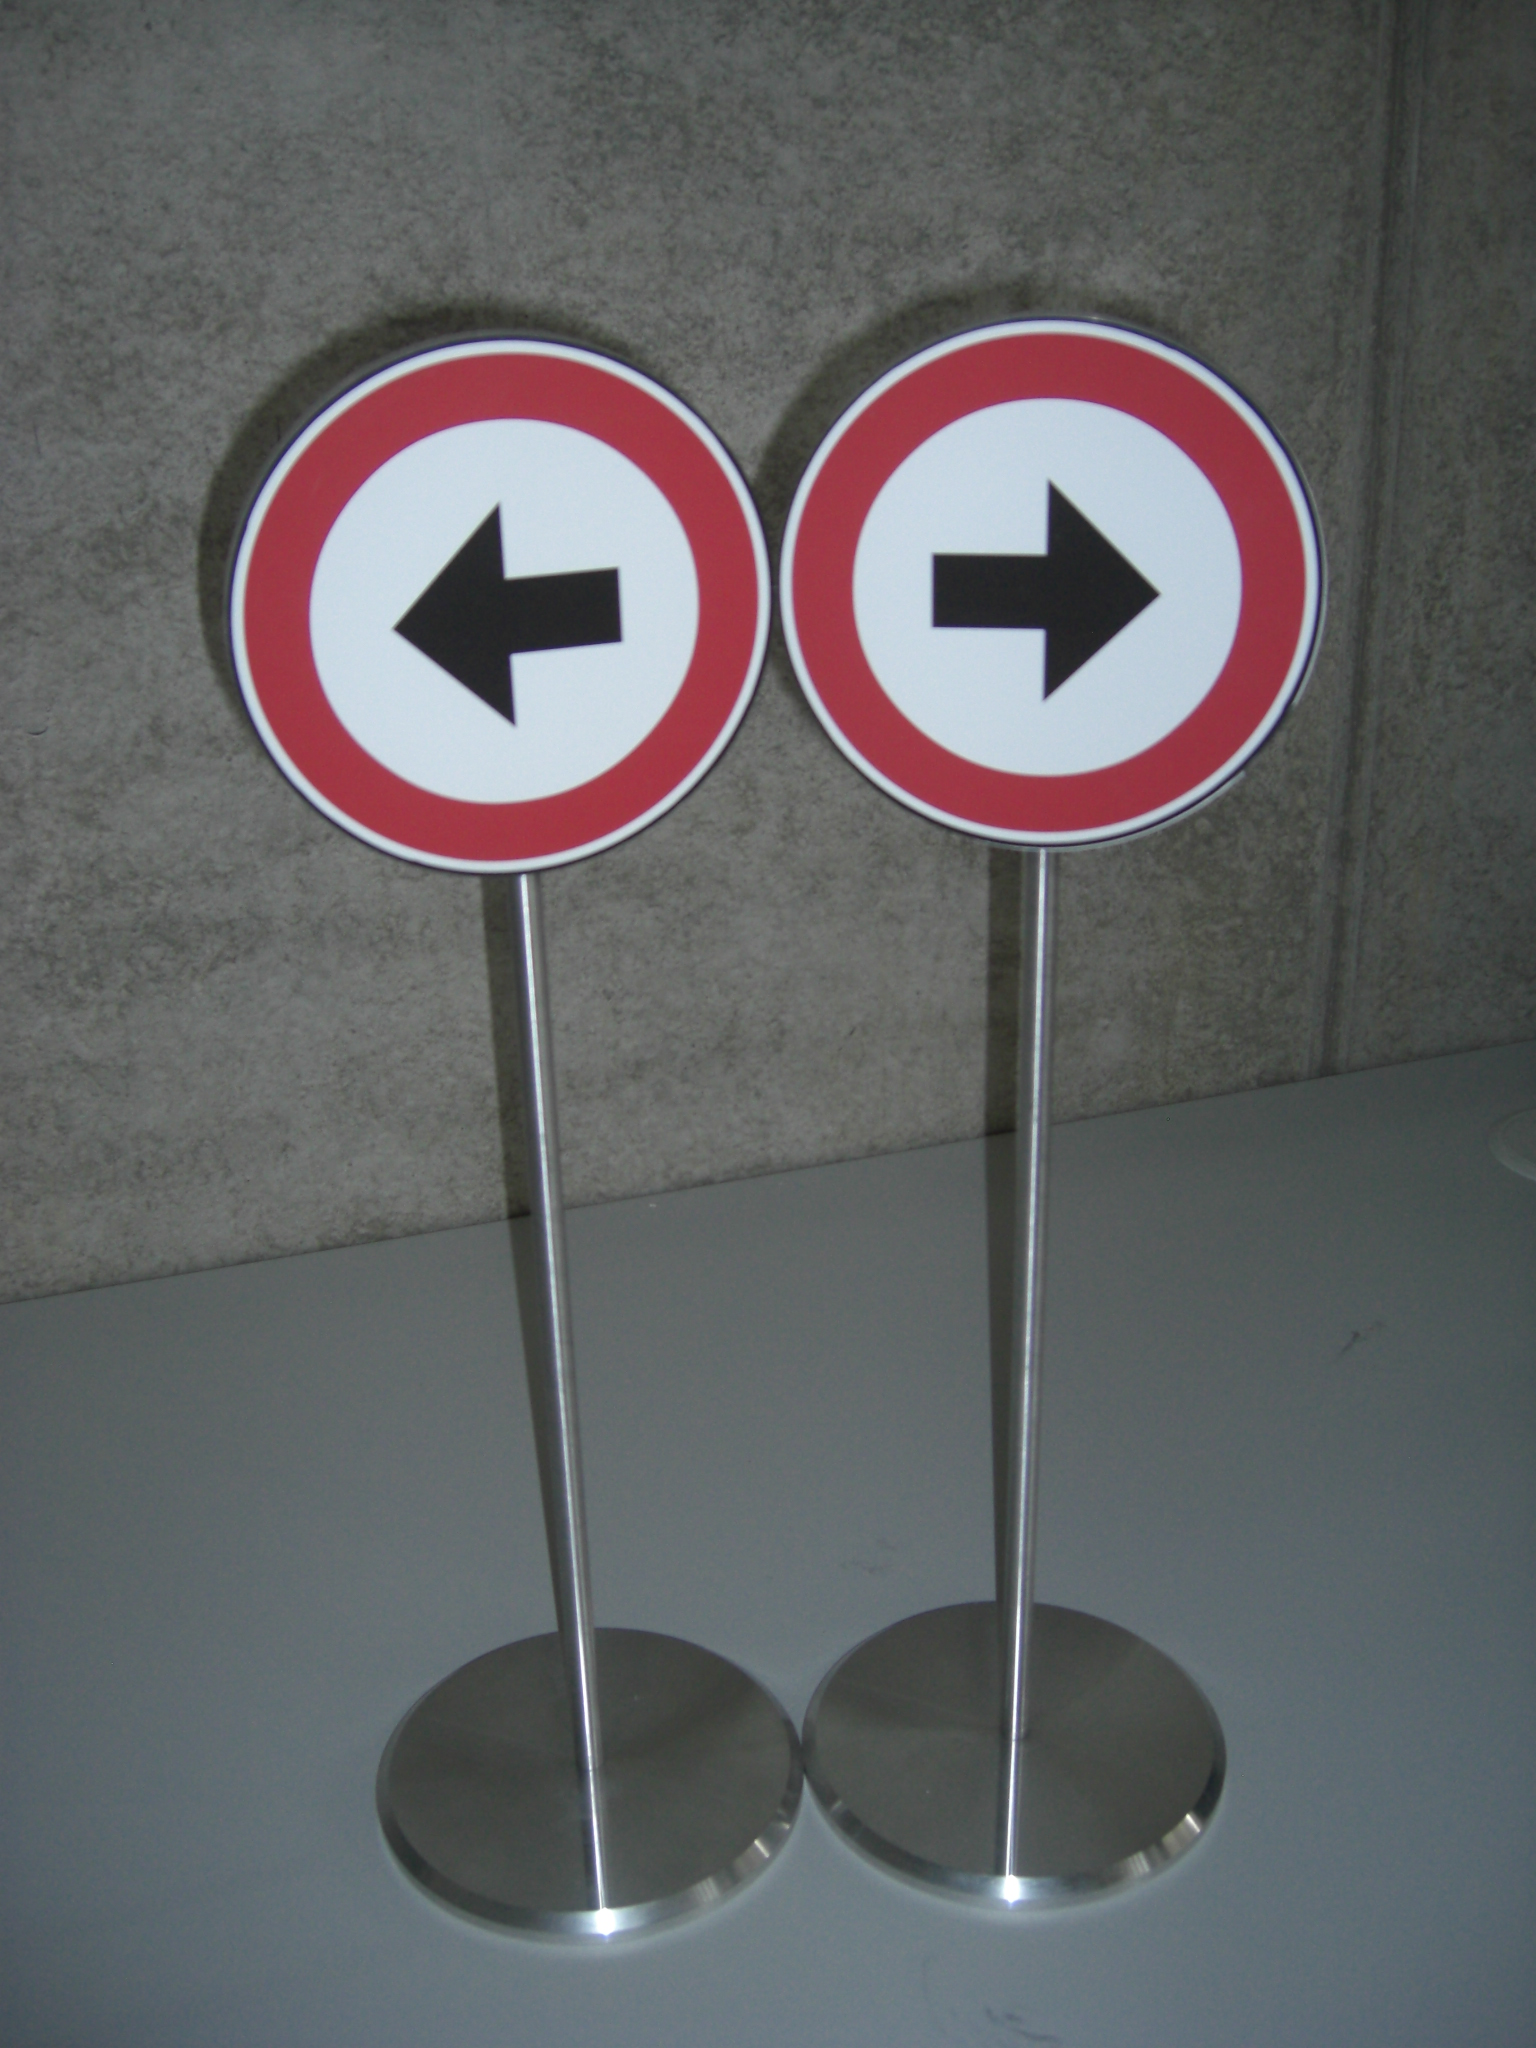
\includegraphics[scale=0.07]{signs.jpg}  & 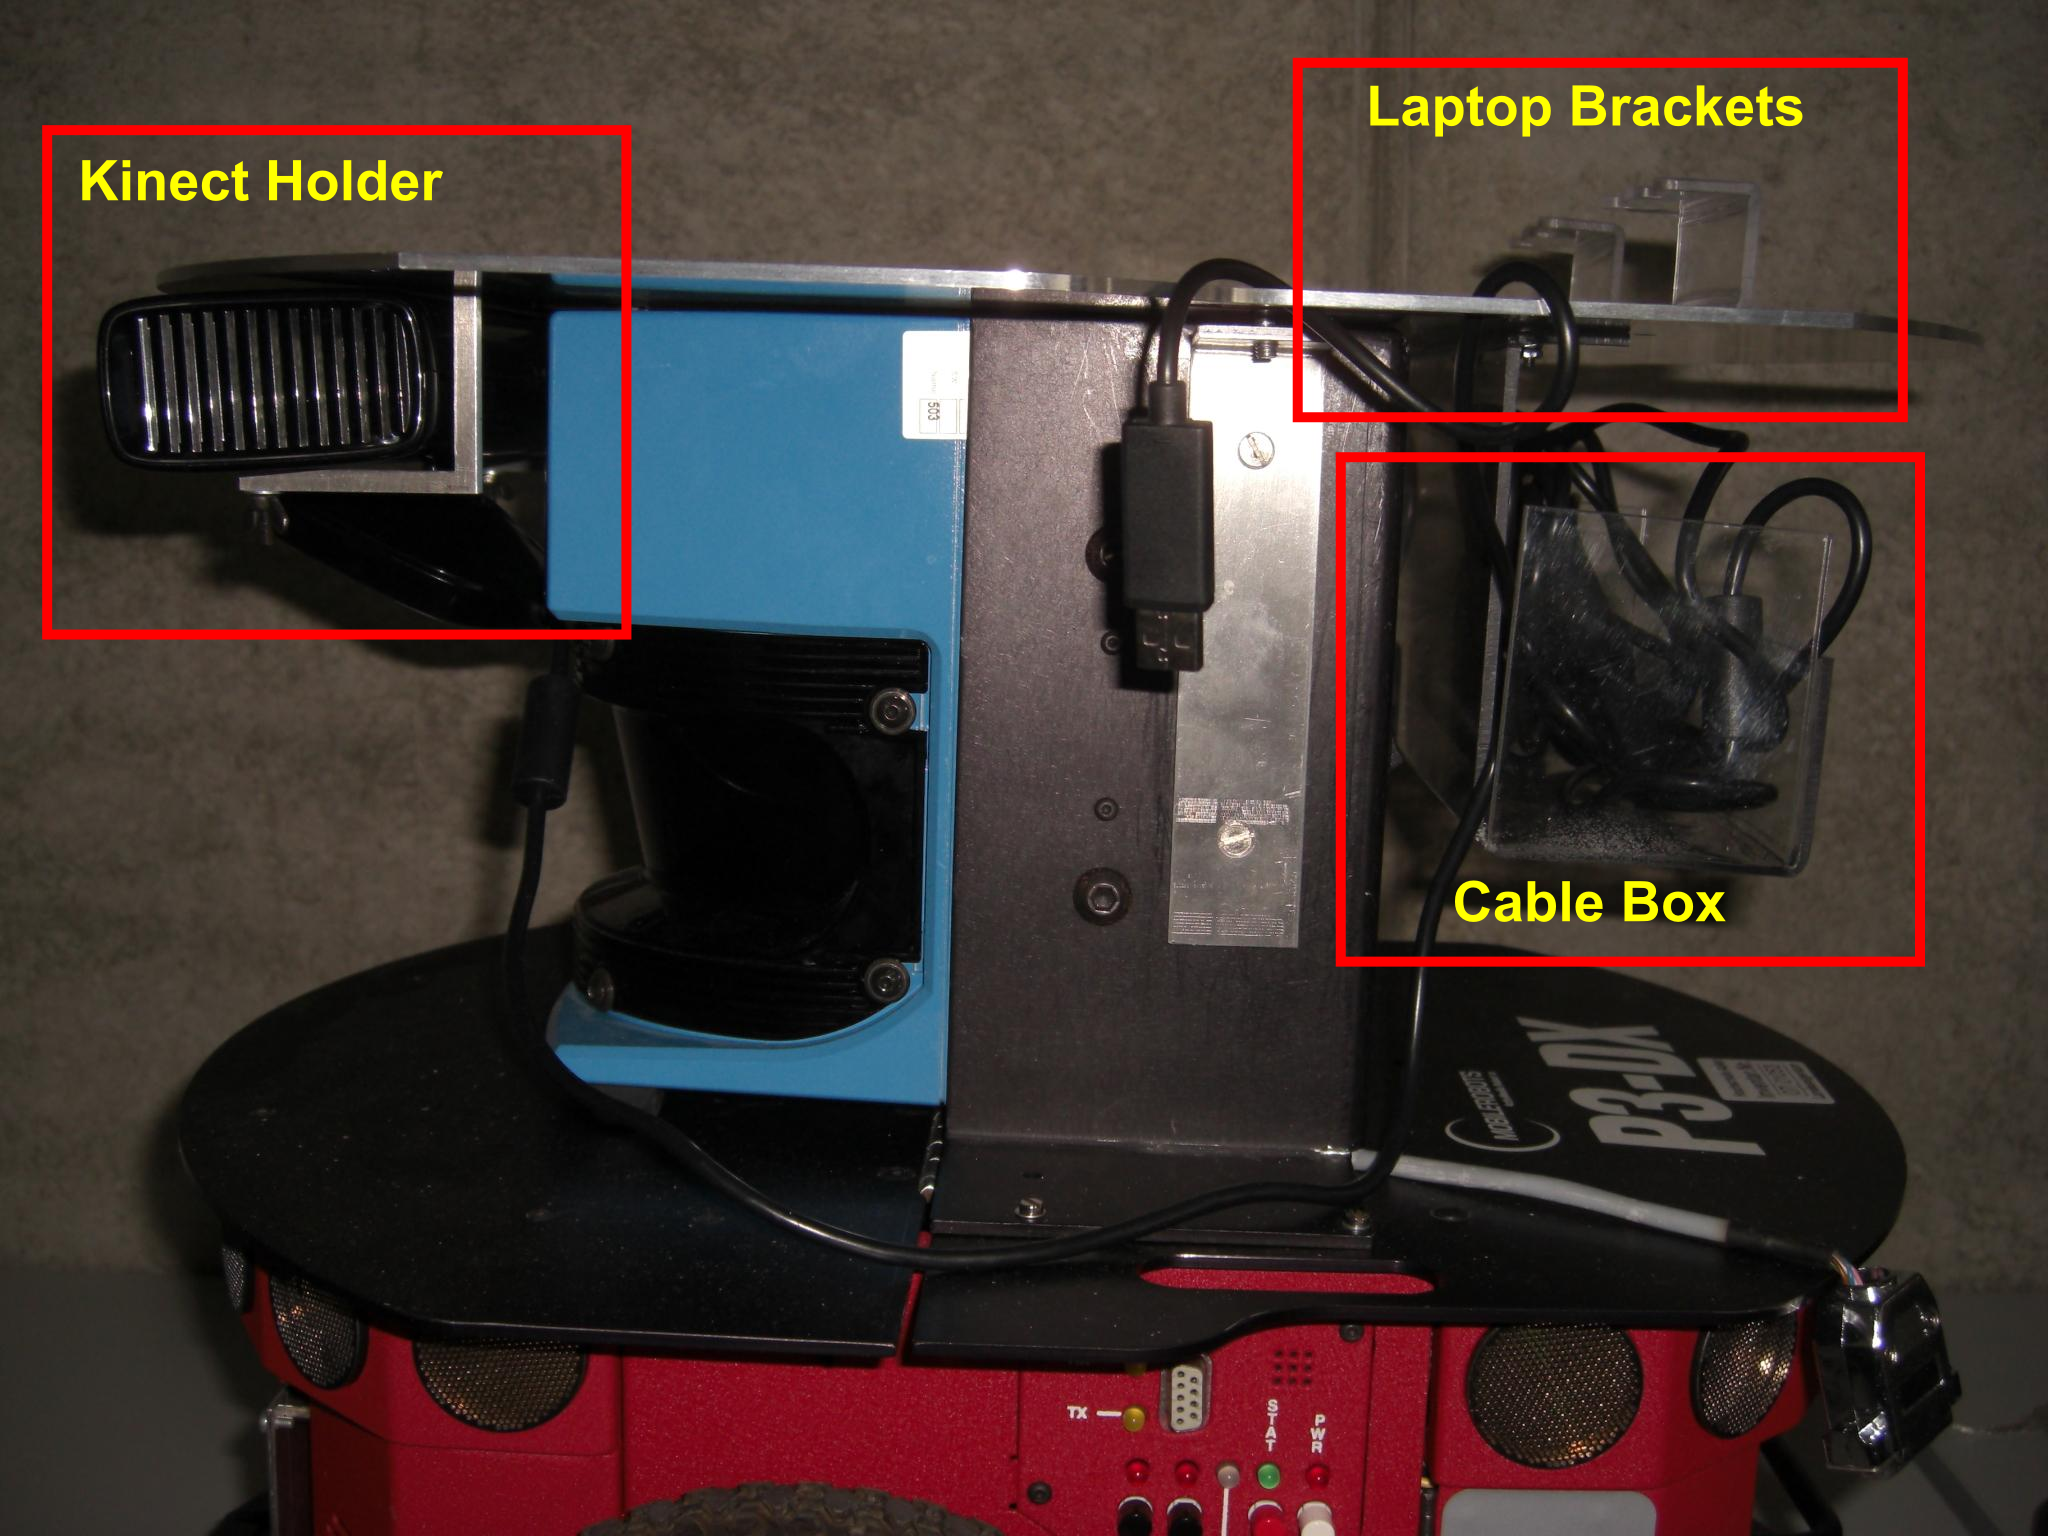
\includegraphics[scale=0.1]{laptop_stand_side.png}\\	
		\end{tabular}
	\end{frame} 
	  
	
	\section{Kinect Analyse} 
	\subsection{Tools}
	
	\begin{frame}{DepthImageAnalyzer (Qt Node)}
		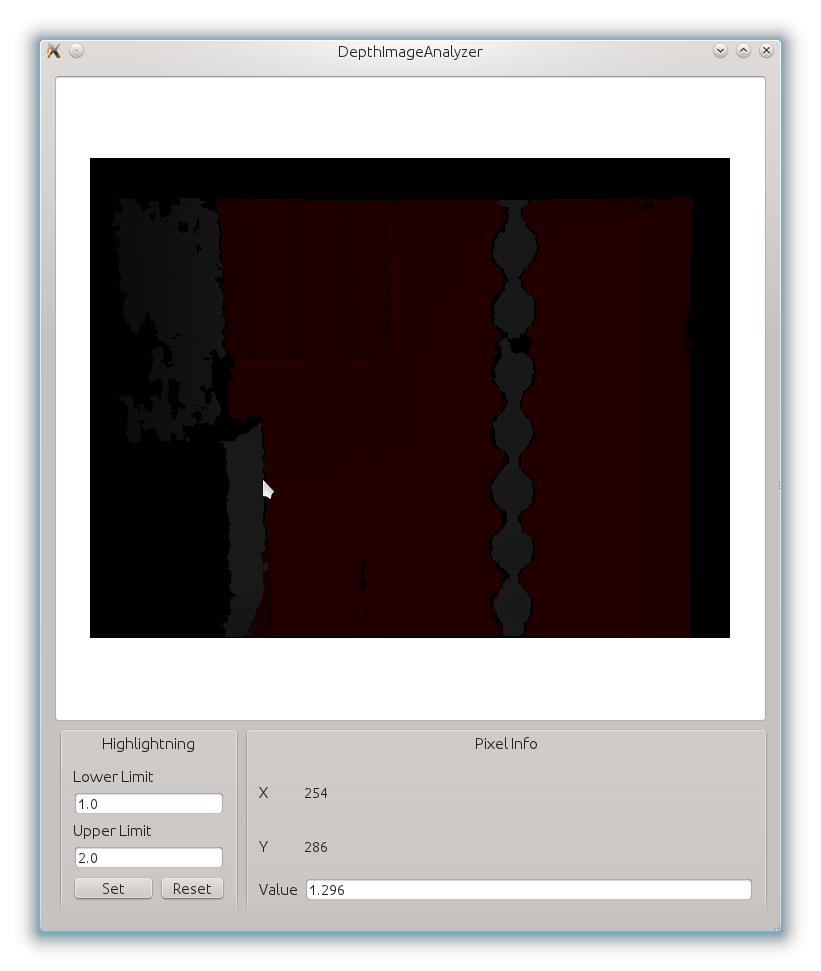
\includegraphics[scale=0.2]{DepthImageAnalyzer.jpg}
	\end{frame}
	
	\begin{frame}{Rviz}
		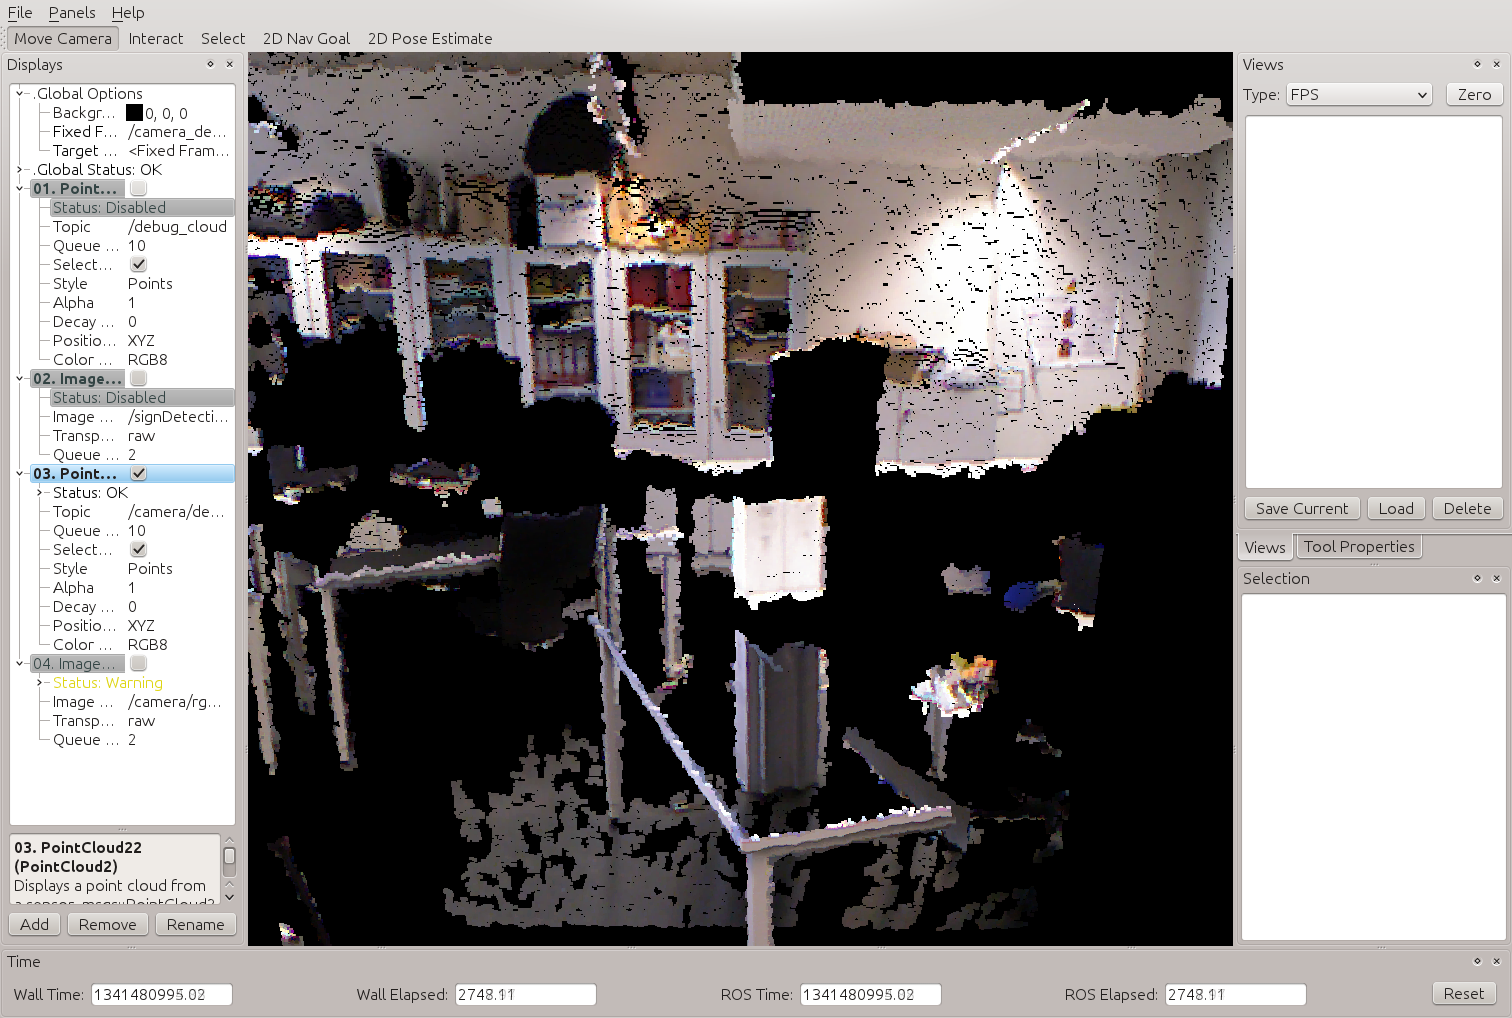
\includegraphics[scale=0.4]{RVizPointCloud.png}
	\end{frame} 
	
	\begin{frame}{Node mit PointCloud}
		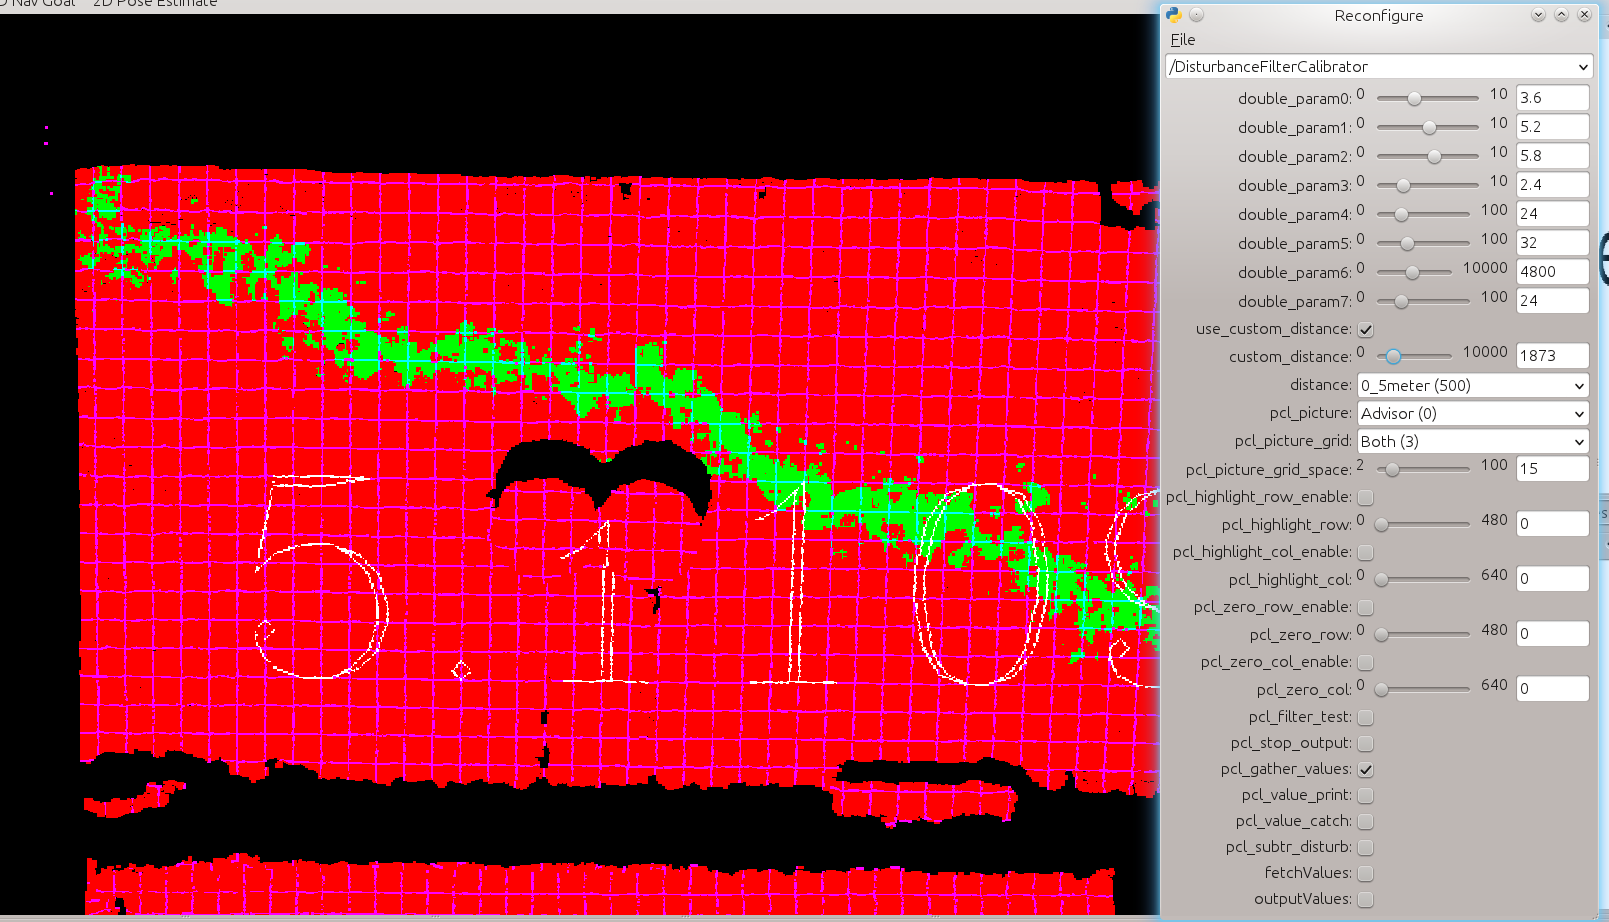
\includegraphics[scale=0.35]{disturbance_filter_calibrator1.png}	
	\end{frame}
	
	
	\subsection{Probleme mit Oberflächen}
		
		
	\begin{frame}{\insertsubsection: Zu Nah}	
		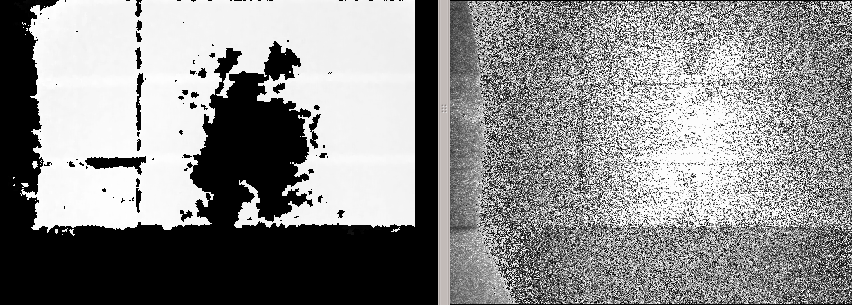
\includegraphics[scale=0.6]{ToClose.png}
	\end{frame}
			
	\begin{frame}{\insertsubsection: Sonneneinstrahlung}	
		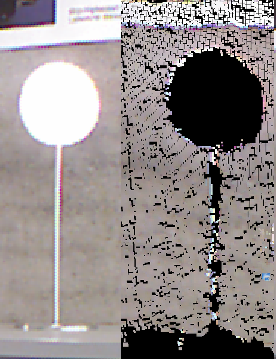
\includegraphics[scale=1.2]{Sun.png}
	\end{frame}
			
	\begin{frame}{\insertsubsection: Spiegelnde Flächen}	
		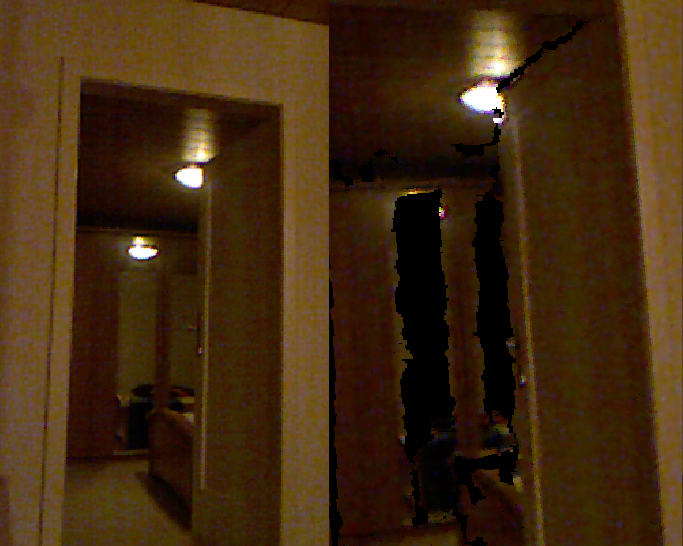
\includegraphics[scale=0.8]{Mirror.png}
	\end{frame}
	
	\begin{frame}{\insertsubsection: Transparente Materialien}	
		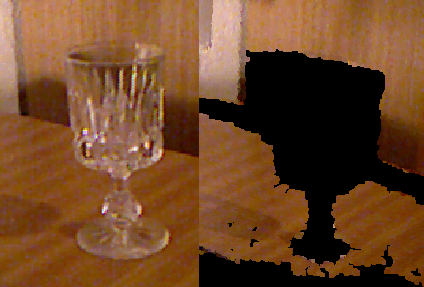
\includegraphics[scale=1]{glas.png} 	
	\end{frame}
	
	\subsection{Ergebnisse}

	
	%%%%%%%%%%%%%%%%%%%%%%%%%%%%%%%%%%%%%%%%%%%%%%%%%%
	%SOFTWARE
	%%%%%%%%%%%%%%%%%%%%%%%%%%%%%%%%%%%%%%%%%%%%%%%%%%
	
	
	\section{Software}  
	\subsection{Bildbeschaffung}
	\subsection{Step Map} 
	  
	\begin{frame}{Vielen Dank für Ihre Aufmerksamkeit}
	    \begin{itemize}
	      \item Dokumentation und Quellcode(comming sooner or later):\\
	      {\small\url{http://radiationlaboratories.blogspot.de/2012/07/online-symbol-recognition-through-data.html}}\\
	       (Shortlink: \url{http://tinyurl.com/OSR-3D-RGB})\\ 
\includegraphics[scale=1]{qrLink.png}
	       
	    \end{itemize}
	\end{frame} 

\end{document}
 